\section{Introduction}
\label{sec:intro}

This sample exercises every package in the stack.
\enquote{Clone and build} is the goal: run \texttt{make} and get a working PDF\@.
Prior work~\autocite{example2024} motivates the setup.
\Cref{sec:method} defines the problem; \cref{sec:results} shows outputs.
\todo[inline]{This file is a kitchen-sink demo.
  Delete it and start writing.
}

\section{Method}
\label{sec:method}

Let $f \colon \R^n \to \R$ be twice differentiable.
We seek
%
\begin{equation}
  \label{eq:argmin}
  x^\star = \argmin_{x \in \R^n}\, f(x).
\end{equation}
%
The solution satisfies
%
\begin{equation}
  \label{eq:cases}
  \nabla f(x^\star) =
  \begin{dcases}
    0        & \text{if } x^\star \in \operatorname{int}(\R^n), \\
    -\lambda & \text{otherwise.}
  \end{dcases}
\end{equation}
%
We define $g \coloneqq \nabla f$ and note
%
\begin{align}
  \|g(x)\|^2 & \leq L \ab(f(x) - f(x^\star)) \label{eq:gradient-bound} \\
  \shortintertext{with}
  L          & \coloneqq \sup_{x} \|\nabla^2 f(x)\|.
  \notag
\end{align}
%
The condition number is $\kappa \coloneqq L / \mu$ where $f$ is $\mu$-strongly convex.
Standard bracket notation from \texttt{physics2}: $\ab|x|$, $\ab[x]$, and $\ab(x + y)$.

\section{Results}
\label{sec:results}

\Cref{fig:objective} shows a \TikZ{} sketch and \cref{fig:convergence} shows a \texttt{pgfplots} chart.

\begin{figure}[h]
  \centering
  \begin{tikzpicture}
    \draw[->] (0,0) -- (3,0) node[right] {$x$};
    \draw[->] (0,0) -- (0,2) node[above] {$f(x)$};
    \draw[thick,domain=0:2.5,smooth] plot (\x, {0.4*(\x-1.2)^2 + 0.3});
    \fill (1.2, 0.3) circle (1.5pt) node[below right] {$x^\star$};
  \end{tikzpicture}
  \caption{A toy objective with a unique minimum at $x^\star$.}
  \label{fig:objective}
\end{figure}

\begin{figure}[h]
  \centering
  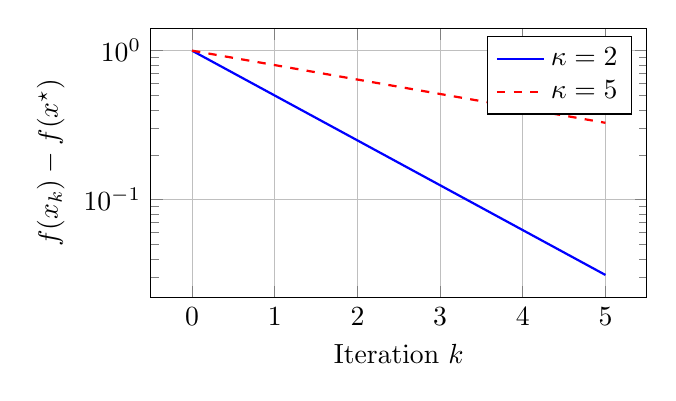
\begin{tikzpicture}
    \begin{axis}[
        width=0.65\textwidth, height=5cm,
        xlabel={Iteration $k$}, ylabel={$f(x_k) - f(x^\star)$},
        ymode=log, grid=major,
        legend pos=north east,
      ]
      \addplot[thick, mark=none, blue] coordinates {
          (0,1) (1,0.5) (2,0.25) (3,0.125) (4,0.0625) (5,0.03125)
        };
      \addlegendentry{$\kappa = 2$}
      \addplot[thick, mark=none, red, dashed] coordinates {
          (0,1) (1,0.8) (2,0.64) (3,0.512) (4,0.410) (5,0.328)
        };
      \addlegendentry{$\kappa = 5$}
    \end{axis}
  \end{tikzpicture}
  \caption{Convergence rate depends on $\kappa$; see \cref{eq:gradient-bound}.}
  \label{fig:convergence}
\end{figure}

\Cref{tab:results} compares two methods.
\todo{Replace with real numbers.}

\begin{table}[h]
  \centering
  \begin{tabular}{lS[table-format=1.2]S[table-format=2.0]}
    \toprule
    {Method} & {Accuracy} & {Runtime (\si{\milli\second})} \\
    \midrule
    Baseline & 0.82       & 12                             \\
    Ours     & 0.91       & 9                              \\
    \bottomrule
  \end{tabular}
  \caption{Placeholder results.}
  \label{tab:results}
\end{table}

As \cref{eq:argmin,eq:cases} and \cref{tab:results} show, the method recovers $x^\star$ with accuracy \num{0.91} in \SI{9}{\milli\second}.
As \textcite{example2024} note, \enquote{further work is needed}.
The speed of light is $c = \SI{3e8}{\metre\per\second}$.
